% Created 2023-10-05 jue 10:53
% Intended LaTeX compiler: pdflatex
\documentclass[11pt]{article}
\usepackage[utf8]{inputenc}
\usepackage[T1]{fontenc}
\usepackage{graphicx}
\usepackage{grffile}
\usepackage{longtable}
\usepackage{wrapfig}
\usepackage{rotating}
\usepackage[normalem]{ulem}
\usepackage{amsmath}
\usepackage{textcomp}
\usepackage{amssymb}
\usepackage{capt-of}
\usepackage{hyperref}
\usepackage{../modern}
\bibliography{./fuentes.bib}
\raggedbottom
\setcounter{secnumdepth}{2}
\author{Luis Eduardo Galindo Amaya (1274895)}
\date{5 de Octubre 2023}
\title{Taller 5. Variables de Ambiente}
\hypersetup{
 pdfauthor={Luis Eduardo Galindo Amaya (1274895)},
 pdftitle={Taller 5. Variables de Ambiente},
 pdfkeywords={},
 pdfsubject={},
 pdfcreator={Emacs 27.1 (Org mode 9.3)}, 
 pdflang={Spanish}}
\begin{document}

\modentitlepage{../images/escudo-uabc-2022-color-cont.png}
\tableofcontents\pagebreak
\datasection{Individual}


\section{Introducción}
\label{sec:orgce1d09b}
Los Sistemas operativos Unix-Like permiten configurar variables de manera que
se puede configurar como funciona la manera en la que se ejecutan los programas 
a lo largo de esta practica aprenderemos como crear, modificar, mostrar y 
eliminar variables de shell. 

\pagebreak

\section{Actividades}
\label{sec:org3515346}
\subsection{Muestre todas las variables que hay en su sesión de trabajo}
\label{sec:orgecd2917}
\begin{itemize}
\item \autocite{0001_P} El comando \texttt{set} escribirá los nombres y valores de todas las variables de shell en la secuencia de ordenación de la configuración regional actual.
\end{itemize}

\begin{verbatim}
set
\end{verbatim}

\begin{figure}[htbp]
\centering
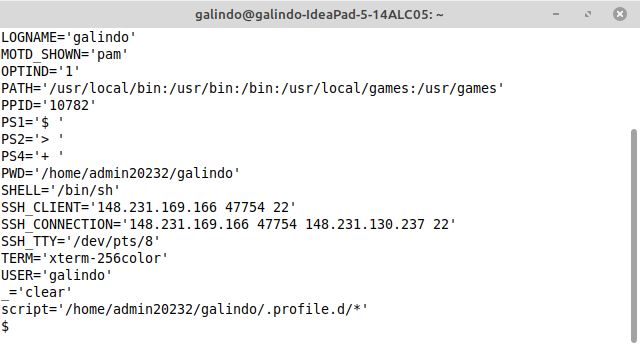
\includegraphics[width=10cm]{img/1.png}
\caption[\texttt{set}]{Salida del comando \texttt{set}}
\end{figure}

\subsection{Muestre solamente las variables de ambiente}
\label{sec:orgeb49436}
\begin{itemize}
\item \autocite{0002_P} Imprime los valores de la(s) VARIABLE(s) de entorno especificada(s). Si no se especifica ninguna VARIABLE, imprime los pares de nombre y valor de todas ellas.
\end{itemize}

\begin{verbatim}
printenv
\end{verbatim}

\begin{figure}[htbp]
\centering
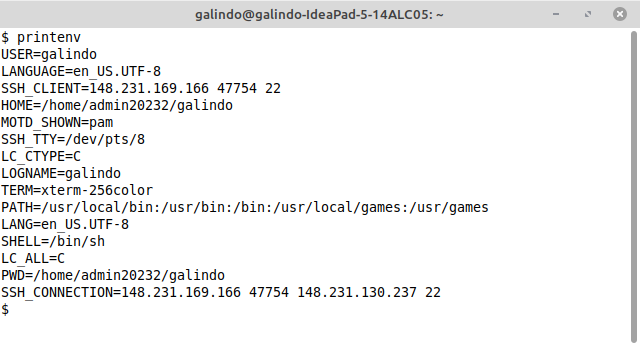
\includegraphics[width=10cm]{img/2.png}
\caption[\texttt{printenv}]{Salidad del comando \texttt{printenv}}
\end{figure}

\subsection{Modifique el valor de una de las variables de ambiente}
\label{sec:org5961707}
\begin{itemize}
\item \autocite{Rainville_2020} Para modificar el valor de una variable en linux utilizarmos \texttt{exoprt}, en el siguiente ejemplo modifico la variable \texttt{USER} del entorno.
\end{itemize}

\begin{verbatim}
export USER=Test
\end{verbatim}

\begin{twoc}
\begin{center}
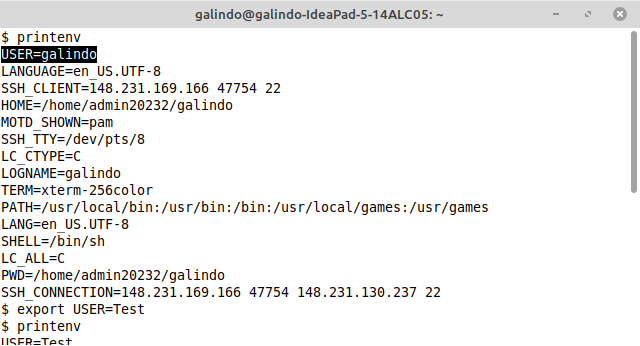
\includegraphics[width=.9\linewidth]{img/3a.png}
\end{center}
\end{twoc}
\begin{twoc}
\begin{center}
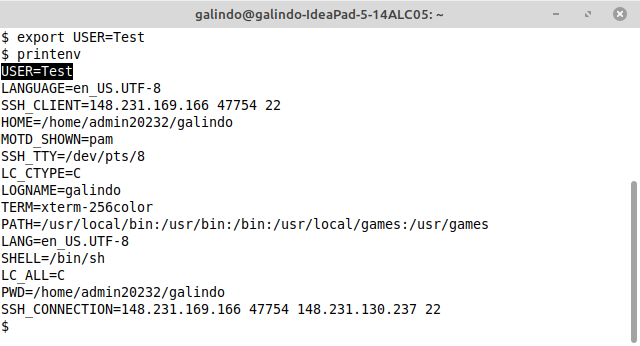
\includegraphics[width=.9\linewidth]{img/3b.png}
\end{center}
\end{twoc}

\subsection{¿Se puede modificar nuestro user name? Si/No ¿por qué?}
\label{sec:org6ce90e4}
\begin{itemize}
\item \autocite{Pablinux_2019} Si, es posible cambiar el user name pero debemos cambiar tambien el UID \texttt{usermod -l nuevo-nombre viejo-nombre} y \texttt{usermod -u UID username}
\end{itemize}
\pagebreak

\subsection{¿Cual es la diferencia entre las líneas de comando \$echo PATH y \$echo \$PATH?}
\label{sec:org7f34952}
\begin{itemize}
\item \texttt{echo PATH} imprime el string 'PATH' en la terminal
\item \texttt{echo \$PATH} imprimer el valor de la varible 'PATH'
\end{itemize}

\begin{figure}[htbp]
\centering
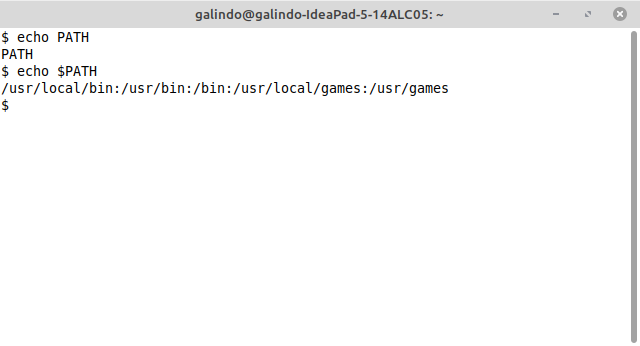
\includegraphics[width=10cm]{img/4.png}
\caption{Salida de los comandos}
\end{figure}

\subsection{Cree una variable de shell con su nombre y asignele su matricula como valor}
\label{sec:org1b416f8}
\begin{verbatim}
mi_nombre="Luis Eduardo Galindo Amaya"
matricula="1274895"
\end{verbatim}

\begin{figure}[htbp]
\centering
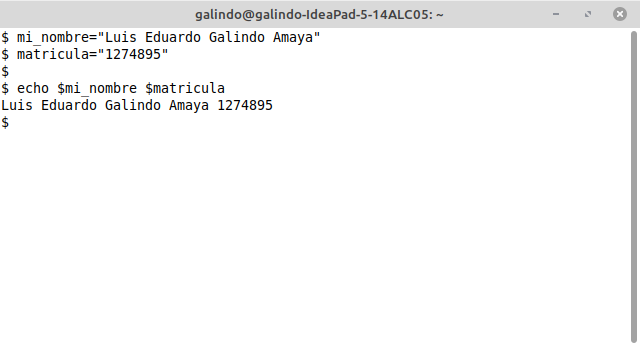
\includegraphics[width=10cm]{img/5.png}
\caption[\texttt{matricula}]{Valor de \texttt{mi\_nombre} y de \texttt{matricula}}
\end{figure}

\pagebreak

\subsection{Cree una variable de ambiente con su nombre y asignele su matricula como valor}
\label{sec:orgc4906a0}
\begin{verbatim}
export MI_NOMBRE="Luis Eduardo Galindo Amaya"
export MATRICULA="1274895"
\end{verbatim}

\begin{figure}[htbp]
\centering
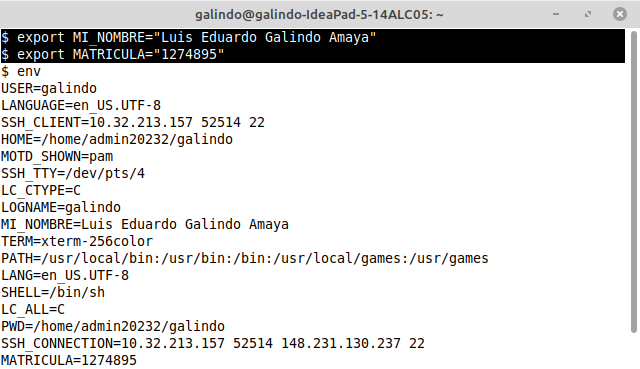
\includegraphics[width=10cm]{img/6.png}
\caption[\texttt{printenv}]{\texttt{printenv} con variables}
\end{figure}

\subsection{Modifique el prompt primario}
\label{sec:org0bd5bb3}
\begin{verbatim}
PS1="PS1>"
\end{verbatim}

\begin{figure}[htbp]
\centering
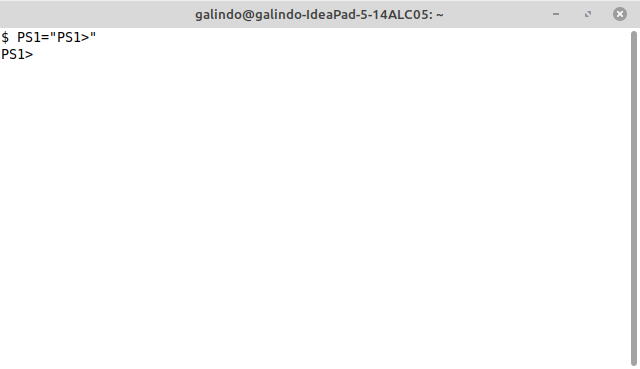
\includegraphics[width=10cm]{img/7.png}
\caption{El prompt primario es el que siempre aparece en la terminal}
\end{figure}

\pagebreak

\subsection{Modifique el prompt secundario}
\label{sec:org98e3d4d}
\begin{verbatim}
PS2="PS2>"
\end{verbatim}

\begin{figure}[htbp]
\centering
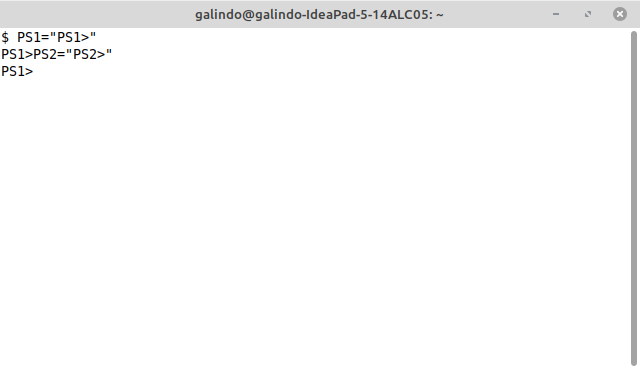
\includegraphics[width=10cm]{img/8a.png}
\caption{Cambiando el valor del prompt secundario}
\end{figure}

\begin{figure}[htbp]
\centering
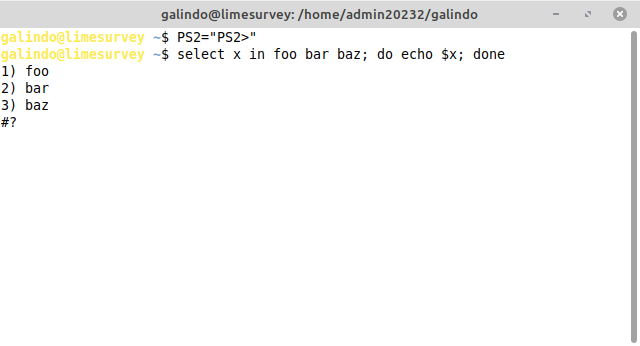
\includegraphics[width=10cm]{img/8.png}
\caption{El prompt secundario aparece con comandos incompletos \autocite{0003_P}}
\end{figure}
\pagebreak

\subsection{Elimine la variable de ambiente que creó en el punto 7.}
\label{sec:org75df835}
\begin{verbatim}
unset MATRICULA
unset MI_NOMBRE
\end{verbatim}

\begin{figure}[htbp]
\centering
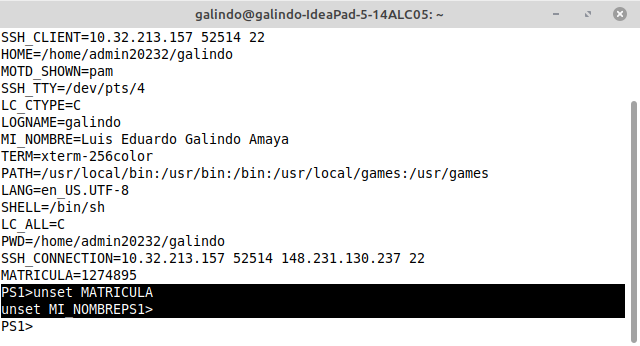
\includegraphics[width=10cm]{img/9.png}
\caption{Eliminado las variables}
\end{figure}

\begin{figure}[htbp]
\centering
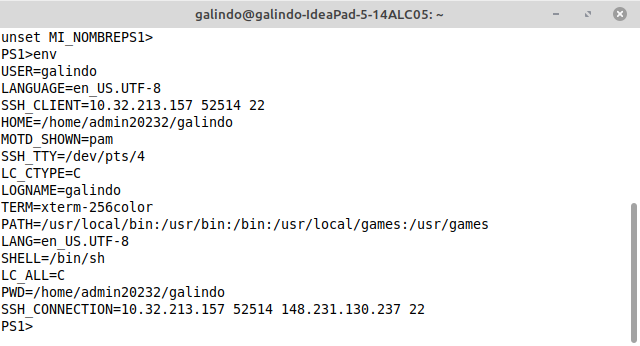
\includegraphics[width=10cm]{img/9b.png}
\caption{las variables ya no aparecen}
\end{figure}

\section{Conclusión}
\label{sec:orge121450}
A lo largo de esta practica aprendí como crear variables de entorno y como 
modificar algunas de las características del sistema operativo, me pareció 
muy interesante como en Unix es posible cambiar como el sistema ejecuta los
programas en ejecución o como cada programa puede cambiar las cosas de un 
proceso a otro. 

\pagebreak

\section{Referencias}
\label{sec:org9b1d6b3}
\printbibliography[heading=none]
\end{document}
